% Niveau :      sup
% Discipline :  Méca

\begin{exercise}{Fluctuation de la durée du jour}{3}{Sup, spé}
{Mécanique,Moment cinétique}{bermudez}


\begin{questions}
    \questioncours Présenter l'analogie entre moment cinétique et quantité de mouvement, et discuter de leur conservation. On fera un tableau pour comparer les différentes grandeurs en jeu dans chaque cas.
    \uplevel{
La durée du jour, $\tau_\text{j}$, actuellement de 24h, fluctue sur des échelles de temps très variées allant de quelques jours sur plusieurs millions d'années. La figure ci-dessous représente la variation de la durée d'une journée depuis les années 1900.

\begin{figure}[H]
    \centering
    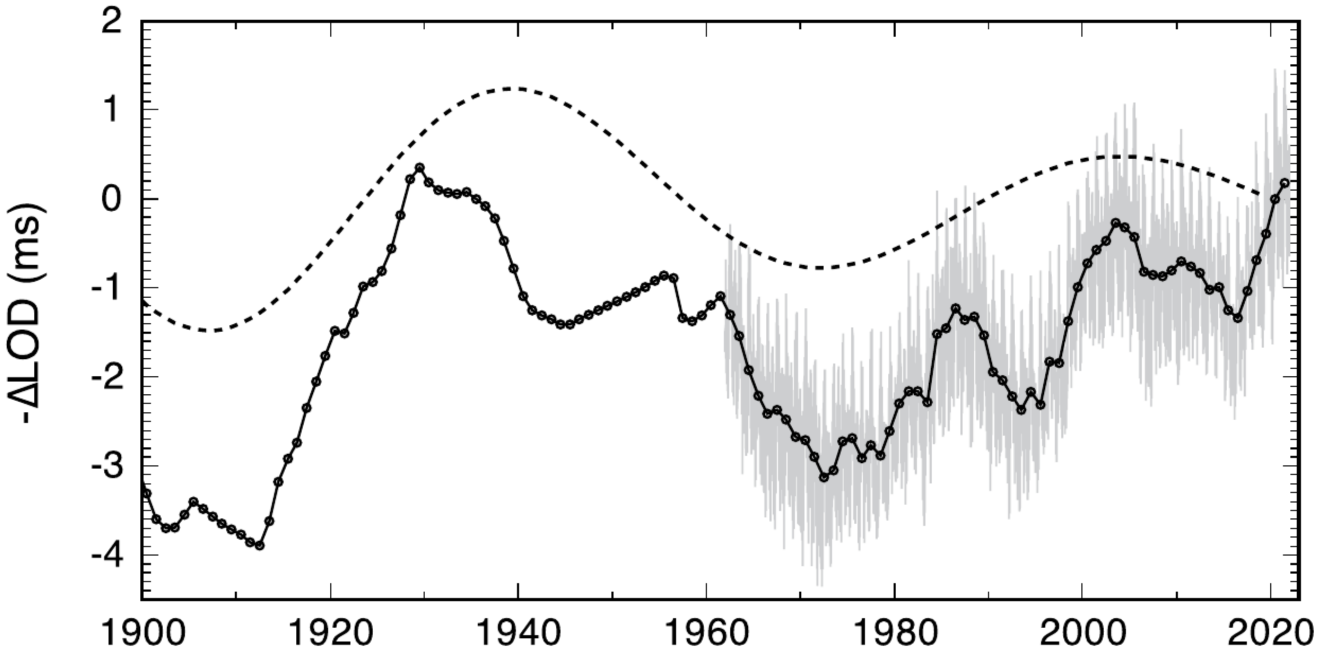
\includegraphics[width=.7\linewidth]{meca/mecasolides/lengthoftheday.png}
    \caption{Variation de la durée d'une journée en millisecondes par rapport aux 24h standard.}
    \label{fig:LOD}
\end{figure}

Il y a plusieurs million d'années, elle était de 22h. Par l'effet du couplage Terre--Lune, elle a augmentée graduellement avec le temps.

Il a été mis en évidence très récemment, que la durée du jour pouvait également fluctuer sur des périodes d'environ 70 ans (en pontillés sur la figure~\ref{fig:LOD}) à cause du renversement de la rotation du noyau interne de la Terre, qui libre de tourner dans le noyau externe, liquide, est presque immobile depuis 2013.

La durée du jour fluctue également sur des échelles de temps plus courtes par couplage entre l'atmosphère et la Terre. Pour des échelles de temps de l'ordre de quelques jours à quelques années (en gris sur la figure~\ref{fig:LOD}), cela est principalement attribué aux courants atmosphériques globaux, comme les alizés (vents d'est, à l'équateur en basse altitude), les vents d'ouest (latitude $30^\circ$, basse altitude) et les jet stream (vents d'ouest aux latitudes $60^\circ$ en haute altitude), qui ont des vitesses qui varient sur des valeurs de l'ordre de 100 km/h typiquement.

\textsf{Problème ouvert :} en utilisant les résultats de la question précédente et à l'aide des données, estimer en ordre de grandeur les quantités suivantes :
}

    \question la fluctuation d'une journée due à l'arrêt de la rotation du noyau interne de la Terre ;
    \question la fluctuation d'une journée due aux courants atmosphériques globaux ;
    \question l'éloignement moyen entre la Terre et la Lune en cm/siècle.
\end{questions}

\paragraph{Données :}(toutes ne sont pas utiles)\\[-2em]
\begin{multicols}{2}
\begin{itemize}
    \item masse de la Terre : $m_\textsc{t} = 6,0\times 10^{24}$ kg ;
    \item masse de la Lune : $m_\textsc{l} = 7,4\times 10^{22}$ kg ;
    \item masse de l'atmosphère : $m_\text{a} = 5,3\times 10^{18}$ kg ;
    \item densité normale de l'air au niveau de la mer : $\rho = 1,3\ \mathrm{kg\cdot m^{-3}}$ ;
    \item densité myenne du noyau interne : $\rho = \SI{12 300}{kg/m3}$ ;
    \item distance Terre--Lune : 384 400 km ;
    \item rayon moyen de la Terre : $R_\textsc{t} = 6371$~km ; 
    \item rayon moyen du noyau interne : $R_\text{n} = 1220$~km ;
    \item constante universelle de gravitation : $G = 6,67\times 10^{-11}$ SI ;
    \item moment d'inertie d'une boule remplie uniformément : $J=\dfrac{2}{5}MR^2$ ;
    \item moment d'inertie d'une sphère creuse : $J=\dfrac{2}{3}MR^2$ ;
    \item moment d'inertie d'un anneau fin : $J =MR^2$.
    \item
\end{itemize}
\end{multicols}
\end{exercise}

\begin{solution}

\plusloin~\\[-2em]
\begin{itemize}
    \item Retrouver la masse de l'atmosphère et de la Terre à partir des données ;
    \item Retrouver les formules littérales des moments d'inertie ;
\end{itemize}

\end{solution}